\documentclass[letterpaper, 10 pt, conference]{ieeeconf}  % Comment this line out if you need a4paper
%\documentclass[a4paper, 10pt, conference]{ieeeconf}      % Use this line for a4 paper

\IEEEoverridecommandlockouts  % This command is only needed if 
                              % you want to use the \thanks command
\overrideIEEEmargins          % Needed to meet printer requirements.


\usepackage{cite}
\let\proof\relax 
\let\endproof\relax 
\usepackage{amsmath, amssymb, amsfonts, amsthm}
\usepackage{graphicx}
\usepackage{subcaption}
\usepackage{float}
\usepackage{textcomp}
\usepackage{subfig}
\usepackage{algorithm}
\usepackage{algpseudocode}
\usepackage[dvipsnames]{xcolor}
\usepackage{booktabs}
\usepackage{multirow}
\usepackage{siunitx}
\usepackage{mwe}

\usepackage[dvipsnames]{xcolor}

\usepackage{mathtools}
\DeclarePairedDelimiter\norm{\lVert}{\rVert}%

\usepackage[capitalize,noabbrev,nameinlink]{cleveref}
\crefformat{equation}{(#2#1#3)}
\Crefname{algocfline}{Algorithm}{Algorithms}
\Crefname{algocf}{line}{lines}
\Crefname{assumption}{Assumption}{Assumptions}
\crefrangeformat{assumption}{Assumptions~#3#1#4-#5#2#6}

\usepackage{amsmath, nccmath}
\usepackage{etoolbox}
\AtBeginEnvironment{bmatrix}{\setlength{\arraycolsep}{1pt}}
\setcounter{MaxMatrixCols}{30} 

% \usepackage{balance}
% \usepackage[%
%     %style=numeric-comp,
%     style=ieee,
%     sorting=none,
%     natbib=true,  % Imitate the natbib package (e.g. using \citet, \citep)
%     % block=ragged,
%     backend=biber,
%     sortcites=true,
%     doi=false,
%     url=false,
%     giveninits=true,
%     maxcitenames=4, %How many people before *choosing* to contract with [et al.]
%     minbibnames=3, %How many authors *at least*  before *inserting* the [et al.]
%     maxbibnames=4, %How many authors *at most*  before *inserting* the [et al.]
%     hyperref
% ]{biblatex}
% \bibliography{refs.bib}

\usepackage{tabstackengine}
\setstackEOL{\cr}

% Commands 
\newcommand{\mbf}{\mathbf}
\newcommand{\bs}{\boldsymbol}
\newcommand{\xdim}{n}
\newcommand{\tdim}{r}
\newcommand{\datadim}{p} 
\newcommand{\state}{\mathbf{x}}
\newcommand{\dstate}{\dot \state}
\newcommand{\bxi}{\boldsymbol{\xi}}
\newcommand{\ith}{~$i^\text{th}$~}
\newcommand{\jth}{~$j^\text{th}$~}
\newcommand{\bThx}{\mathbf{\Theta(x)}}
\newcommand{\bXi}{\mathbf{\Xi}}
\newcommand{\bdX}{\mathbf{\dot{X}}}
\newcommand{\param}{\theta}
\newcommand{\bsig}{\bs{\sigma}}
\newcommand*{\vertbar}{\rule[-1ex]{0.5pt}{2.5ex}}
\DeclareMathOperator*{\argmax}{argmax}
\DeclareMathOperator*{\argmin}{argmin}
\newcommand*{\red}{\textcolor{red}}
\newcommand*{\blue}{\textcolor{blue}}
\newcommand*{\violet}{\textcolor{violet}}
\newcommand{\david}[1]{\textcolor{blue}{[David: #1]}}
\newcommand{\somi}[1]{\textcolor{teal}{[Somi: #1]}}

\renewcommand{\algorithmicrequire}{\, \, \, \, \textbf{Input:}}
\renewcommand{\algorithmicensure}{\, \, \, \,  \textbf{Output:}}

\newcommand{\rotvert}{\rotatebox[origin=c]{90}{$\vert$}}
\newcommand{\rowsvdots}{\multicolumn{1}{@{}c@{}}{\vdots}}


\makeatletter
\let\oldnorm\norm
\def\norm{\@ifstar{\oldnorm}{\oldnorm*}}
\makeatother

\newtheorem{remark}{Remark}
\newtheorem{definition}{Definition}
\newtheorem{proposition}{Proposition}
\newtheorem*{proposition-non}{Proposition}
\newtheorem{problem}{Problem}



\graphicspath{ {./images/} } 

% ================================================== % 
% front matter 
% ================================================== % 

\title{\LARGE \bf
Game Theoretic Spacecraft Pursuit Evasion with Fictitious Play
} 

\author{
Junette Hsin$^{1}$ and 
Luis Sentis$^{1}$ 
% <-this % stops a space
% \thanks{*This work was not supported by any organization}% <-this % stops a space
\thanks{$^{1}$Departments of Aerospace Engineering \& Engineering Mechanics and $^{2}$Electrical and Computer Engineering,
        University of Texas at Austin, \{{\tt\small jhsin, lsentis\}@utexas.edu}}%
}
 
\begin{document}

\maketitle 

% \vspace{-10em}

\thispagestyle{empty}
\pagestyle{empty}


% ================================================== % 
\begin{abstract}

We use techniques from celestial mechanics and differential game theory to find optimal trajectories for the non-cooperative spacecraft pursuer-evader game. We compare employing mixed strategies with using deterministic pure strategies and completely random strategies and show results. 

\end{abstract}

% ================================================== % 
% contents 
% ================================================== % 

\section{Introduction}
\label{sec:intro}
Multi-agent systems are increasingly prevalent in space. 
% 
From satellite constellation coordination to autonomous collision avoidance, engineers must design systems that can manage the actions and trajectories of other objects in space while completing mission goals. 
% 
The cooperative multi-agent problem has been extensively studied, which solves for the motion of all agents toward a common objective. 
% 
% Classic cooperative scenarios include docking \red{cite}, communication networks \red{cite}, and 
% 
However, as international competition creates an increasingly crowded field in space, adversarial interactions must be considered. 
% 
% The cooperative problem has been extensively studied, such as in rendezvous and proximity operations problems . 
% with two active spacecraft or with one active and one passive spacecraft 
% has been extensively researched. 
% but the noncooperative problem has received less attention. 
In the noncooperative multi-agent problem, each agent must complete its own objective, such as following a reference trajectory, while defending against attacks or factoring in adversarial behavior from the other agent.
% 
% The 2-player case can be formulated as a two-sided optimization problem.  
% % 
% Disruptions are of particular concern to critical satellite missions. For example, missile attacks on satellites have created debris swarms with low orbital decay rates. Much attention has been directed to tracking artificial satellites as part of space domain awareness, but there is interest in disrupting satellite activities without creating additional debris. 
% This paper assumes that   

% - missile attacks on satellites have created orbital debris
% - space domain awareness
% - there is desire to disrupt satellite activities without creating additional orbital debris
% - passive maneuvers on satellites completing missions
% 
Under these circumstances, game theory is uniquely suited for modeling the strategic interactions of rational agents with competing objectives in complex environments.
An autonomous spacecraft can make decisions to fulfill its own mission objective, such as following a reference trajectory, while factoring in the non-cooperative behavior of other actors.

Game theory has been used in motion planning for robotic systems in which the game is formulated as a multi-agent trajectory optimization problem.
% Compared with single-agent trajectory optimization problems, the methods for solving multi-agent problems are limited as only specialized cases can be solved exactly \red{cite}, although 
Methods for solving such games are limited compared to single-agent problems due to computational challenges \red{cite}, though 
    % - cite: Bolei Di and Andrew Lamperski. Newton’s method and differential dynamic programming for unconstrained nonlinear dynamic games. In Proceedings of the Conference on Decision Making and Control (CDC). IEEE, 2019.
advances in computational methods have yielded progress \red{cite}. 
Extending such methods to the dynamic environment of space presents additional challenges, but 
% particularly for multi-agent systems with competing objectives. 
% and they often consider systems that work to achieve a common goal rather than truly autonomous agents.
% 
% a growing body of research seeks to examine 
research interest in examining autonomous spacecraft systems through a game theoretic framework continues to grow, with 
% such methods 
% Autonomous agents need algorithms 
% Autonomous agents need algorithms to complete their own mission objectives in the presence of 
% for applications such as 
% Applications for such algorithms include 
applications in  
collision avoidance \cite{bombardelli2015optimal}, trajectory design with unknown disturbances \cite{olympio2010designing}, and pursuit and evasion games \cite{pontani2009numerical, stupik2012optimal}.    
% 

% Whereas 
% 
In this work, we focus on developing methods for the non-cooperative spacecraft pursuit-evasion game.
% where the objective of the first agent is to capture the other agent, and the objective of the second agent is to follow a reference trajectory while evading capture. 
The objective of one agent is to follow a reference trajectory while evading capture, and the objective of the second agent is to capture the first agent. 

Previous work has posed the pursuit-evasion game as a mass-optimal zero-sum differential game, finding open loop strategies using PMP \cite{vaseghi2008advanced}. However, the indirect formulation results in time-optimal solutions which require that both spacecraft have always on-thrust, an inefficient method of control \cite{venigalla2021multi}. 
% 
\cite{feng2024method} propose a hierarchical structure model that leverages differential game theory to address the orbital pursuit-evasion dilemmas encountered by spacecraft clusters, incorporating task assignment optimization and saddle point solutions through advanced algorithms \cite{feng2024method}. 
% 
\cite{li2024orbital} extends this by introducing a linear-quadratic differential game approach for orbital pursuit-evasion-defense scenarios, offering insights into multi-player engagements where a defender spacecraft protects an evader from interception \cite{li2024orbital}. 
% 
Additionally, \cite{bian2023control} focus on three-party engagements in low earth orbit, utilizing differential game theory to develop control strategies for scenarios involving an attacker, defender, and target spacecraft, with the attacker maneuvering between evading the defender and pursuing the target \cite{bian2023control}. 
% 
Further, \cite{feng2024method} tackle the pursuit-evasion problem along elliptical orbits, providing a precise gradient method to solve the associated differential equations and demonstrating its efficacy in orbital engagements \cite{pang2024solving}. 
% 
Finally, \cite{wei2023two} introduce hierarchical guidance laws for a pursuer in an orbital pursuit-evasion-defense game, emphasizing the trade-offs between conservative and radical strategies in maneuvering around a defender to minimize pursuit time \cite{wei2023two}. 
% 
These advancements in game-theoretic approaches are critical for the development of autonomous spacecraft capable of complex decision-making in highly dynamic and contested orbital environments. 

\begin{figure}[t!]
    \centering
    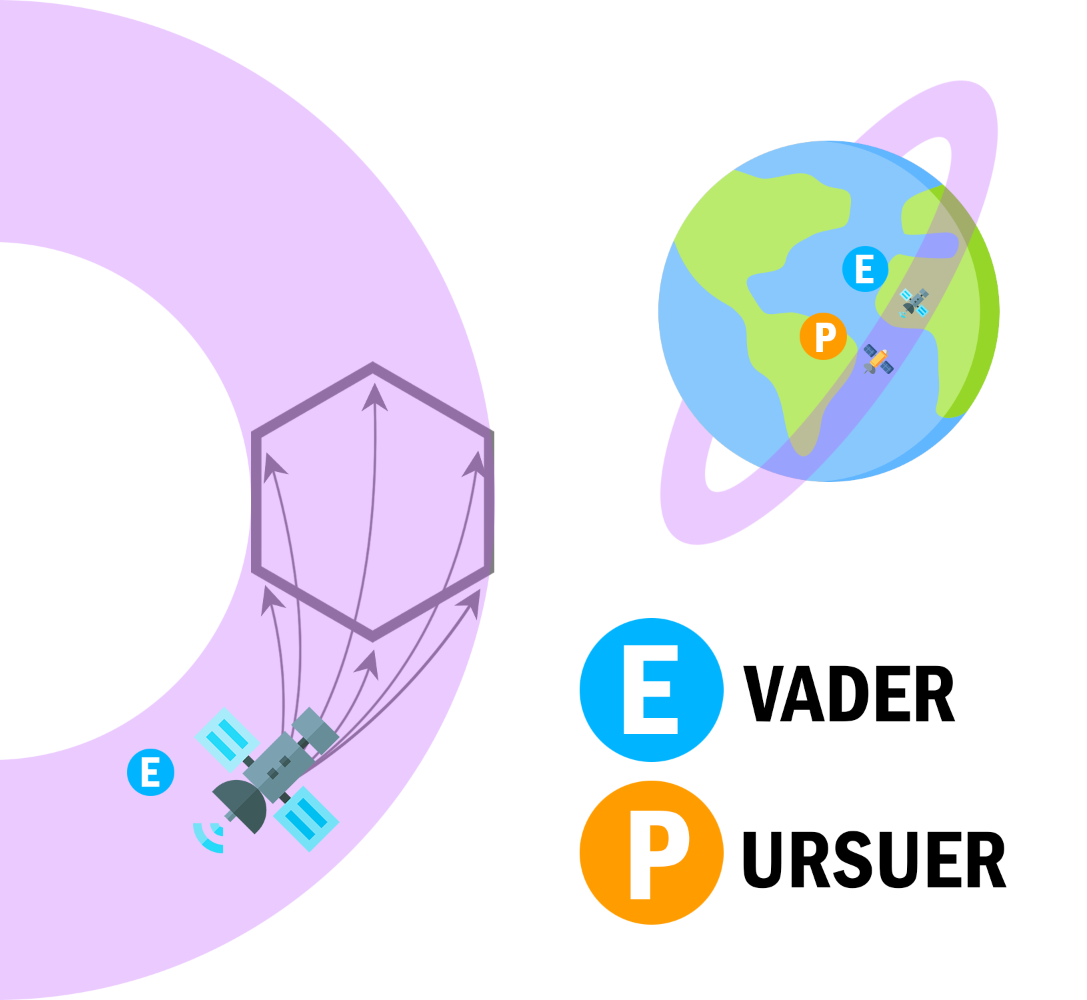
\includegraphics[width=0.9\linewidth]{images/evader_pursuer_diagram.png}
    \caption{Evader and Pursuer diagram}
    \label{fig:evader_pursuer_diagram}
\end{figure}
% \blue{
% The aforementioned approaches use classic game theory approaches to find the Nash equilibrium, or saddle point solution to a differential game. However, equilibrium solutions to trajectory games do not always exist, and deterministic actions can be exploited by an opponent \cite{peters2022learning}. In pure strategies, players are bound to deterministic behavior, and the evader is captured.
% } 

The aforementioned approaches find deterministic strategies by finding the Nash equilibrium, or saddle point solution to a differential game. 
% Equilibrium solutions 
The Nash equilibrium is a situation where no player could gain by changing their own strategy (holding all other players’ strategies fixed). 
However, equilibrium solutions do not always exist as existing methods are either restricted to specialized cases or extend methods from static games without exploiting time-varying dynamics \cite{di_newtons_2019}.  
Crucially, the solution strategies converge onto deterministic strategies which may be exploited by opponents \cite{peters2022learning}. 


% We seek to find optimal trajectories for the non-cooperative spacecraft zero-sum pursuer-evader game subject to orbital dynamics constraints. We assume that the evading spacecraft follows a reference orbit for a designated mission, such as providing telecommunication services or taking images of a specific location at a critical time. In contrast, the mission of the pursuing spacecraft is to disrupt the evader.  

% Pursuit evasion games for spacecraft largely considers two scenarios: interception and rendezvous. Interception is when the pursuer targets the same final location as the evader at some future point in time, and rendezvous is when the pursuer attempts to intercept and match its final velocity with the evader as well. Interception includes kinetic and explosive impacts which can create undesirable large amounts of debris. This paper addresses a rendezvous scenario in the interest of attacking or protecting space assets in ways that do not generate excessive space debris.

In this work, we leverage a formulation of lifted games over multiple trajectory candidates, which admit a natural class of high performance mixed strategies. 
These contributions enable efficient and reliable online trajectory planning for autonomous agents in noncooperative settings, such as the tag example of Figure 1. 
We validate our methods in a suite of Monte Carlo studies, in which we demonstrate that lifting gives rise to mixed strategies as shown in Figure 1(b), providing a significant competitive advantage in both open-loop and receding-horizon play. Our method’s reliable convergence and its ability to explicitly account for constraints enables training from scratch within only a few minutes of simulated self-play. 
Once fully trained, learning can be disabled and our method generates mixed strategies within 2 ms for the tag example in Figure 1.
 

% We constrain the range of motion for the pursuer and evader to an orbital tube whose cross-section is a 6-sided polygon. At each iteration of the planning period, the evader and pursuer target the vertices of the polygon centered at a future point along the reference trajectory. The stage costs of the discretized trajectories to each vertex are computed, averaged, and combined in a 2-player cost bimatrix for the pursuer and evader. We solve the simplex linear program associated with a zero sum game, compute the mixing weights which act as a probability distribution, and sample from the distribution to select a trajectory for each player. We repeat this process to propagate the game state forward. 


% A framework uniquely suited for determining optimal strategies for competing agents is game theory. Game theory is the mathematical study of strategic interactions, and existing game theoretic approaches to multi-agent spacecraft maneuvers include finding deterministic closed-loop \cite{desilva2020} and open-loop \cite{vaseghi2008advanced} Nash equilibrium solutions. In \cite{desilva2020}, the rendezvous problem between two active spacecraft is formulated as a two player nonzero-sum differential game. LQ cooperative and noncooperative differential algorithms are applied to state-dependent Riccati equations (SDRE) describing the game dynamics to obtain a closed-loop feedback control law. Finally, a multiplayer sequential game strategy is synthesized to extend the control law to the relative motion synchronization of multiple vehicles. 




% 



 

% \section{Related Work}
% \label{sec:related_work} 
% \input{sections/related_work}


% ================================================== % s
\section{Problem Formulation}
\label{sec:prob_form}
Consider a system consisting of two autonomous spacecraft in orbit. The evolution of the state $\boldsymbol{x}_i \in \mathbb{R}^n$ for each agent is characterized by its equations of motion, $F$, and its control input, $\boldsymbol{u}_i \in \mathbb{R}^m$ 
% 
\begin{equation} 
    \boldsymbol{x}_i(t_{ k+1 }) = F\big( ( \boldsymbol{x}_i (t_k), \boldsymbol{u}_i(t_k) \big). 
\end{equation} 
% 
We define the state $\boldsymbol{x}_i$ as the Cartesian position and velocity with respect to an Earth-centered inertial frame at discrete timestep $t_k$.
For the dynamics $F$, we use Kepler’s laws to predict the future orbital position of each spacecraft given its current state $\boldsymbol{x}_i$ and time of flight from $t_k$ to $t_{k+1}$ \cite{sims1997preliminary}. 
% and $\Delta$V change.
The control input $\boldsymbol{u}_i$ is the instantaneous velocity change at the beginning of a propagation arc due to an impulsive thrust maneuver, commonly known as a $\Delta$V maneuver.
% This approach is known as the Sims Flanagan model for orbit trajectory optimization \red{cite}.
The objective of one spacecraft, the evader, is to stay within the orbital bandwidth of a reference trajectory while avoiding interception.
The other spacecraft, the pursuer, seeks to intercept the evader. 
% At this stage, we do not factor in sensor uncertainty and estimation, and we assume that each agent has perfect knowledge of the state of the other agent and thus can incorporate open-loop information structures.

We use model-predictive control (MPC) to formulate a finite-horizon trajectory problem for each agent that also considers the strategic behavior of the other agent.
MPC finds the optimal set of control commands and trajectories based on the system model and objective function over a finite time window, repeating the computation process with a shifting horizon. 
In game-theoretic MPC, the Nash equilibrium solution characterizes optimal trajectories for each agent. Each agent follows its optimal trajectory before the equilibrium is re-computed, repeating the process with a shifting time horizon. 


The pursuit evasion finite-horizon trajectory optimization problem can be modeled as a zero-sum differential game
% 
\begin{subequations}
    \begin{alignat}{2}
    &\!\min_{ \boldsymbol{u}_1 } & \qquad & J( \boldsymbol{u}_1, \boldsymbol{u}_2 ) \label{eq:} \\
    &\text{s.t.}                 &        & \boldsymbol{x}_1( t_{k+1} ) = F\big( ( \boldsymbol{x}_1 (t_k), \boldsymbol{u}_1(t_k) \big) \label{eq:} \\
    &                            &        & \boldsymbol{x}_1 \in \mathcal{F} \label{eq:}
    \end{alignat}
\end{subequations}
% 
\begin{subequations}
    \begin{alignat}{2}
    &\!\max_{ \boldsymbol{u}_2 } & \qquad & J( \boldsymbol{u}_1, \boldsymbol{u}_2 ) \label{eq:} \\
    &\text{s.t.}                 &        & \boldsymbol{x}_2( t_{k+1} ) = F\big( ( \boldsymbol{x}_2 (t_k), \boldsymbol{u}_2(t_k) \big) \label{eq:} \\
    &                            &        & \boldsymbol{x}_2 \in \mathcal{F} \label{eq:}
    \end{alignat}
\end{subequations} 
% 
where $ J $ is the objective cost function and $ \mathcal{F} $ is the set of feasible trajectories within the orbit bandwidth. 
We seek a saddle point solution to the differential game; at a saddle point each agent will worsen its outcome if it modifies its strategy. If the pursuer is minimizing, a saddle point or Nash equilibrium solution will be found when 

\begin{equation}
    J( \boldsymbol{u}_1, \boldsymbol{u}_2^* ) \leq J( \boldsymbol{u}_1^*, \boldsymbol{u}_2^* ) \leq J( \boldsymbol{u}_1^*, \boldsymbol{u}_2 ). 
\end{equation}


However, a Nash equilibrium solution to the differential game may not exist, and deterministic strategies may still be exploited by an opponent. 
Worse, non-uniqueness implies that even if an agent finds an equilibrium, the opponent’s predicted Nash trajectory may not be representative of its true strategy.
 



% Consider a system characterized by unknown dynamics 
% % 
% \begin{align}
%     \label{eq:prob}
%     \dot{\boldsymbol{x}}(t) &= f( \boldsymbol{x}(t), \boldsymbol{u}(t) ), 
% \end{align} 
% %
% where $t \in \mathbb{R}$, $\boldsymbol{x}(t) \in \mathbb{R}^n$ denotes the state of the system at time $t$, 
% and $\boldsymbol{u}(t) \in \mathbb{R}^m$ the control input. 
% % 
% We presume that $f : \mathbb{R}^{n} \times \mathbb{R}^{m} \to \mathbb{R}^{n}$ in \eqref{eq:prob} is unknown, meaning we have no prior knowledge of the system dynamics. 
% % 
% In many systems, $f$ is a \textit{simple} function in that only a sparse set of quantities, e.g. damping or inertial forces, contribute to the dynamics \cite{wentz_derivative-based_2023}.
% % 
% We assume that we have access to a dataset $\boldsymbol{X}$ consisting of a sequence of $r \in \mathbb{N}$ state measurements corrupted by noise and control inputs $\boldsymbol{U}$ 
% % 
% taken at discrete times 
% $t_{1}, t_{2}, \ldots, t_{r}$,
% % 
% given by
% \begin{equation}
% \label{eq:dataset}
%     \begin{split}
%         \boldsymbol{X} & = \lbrace \boldsymbol{x}(t_1) + \boldsymbol{\epsilon}_{1}, \boldsymbol{x}(t_2) + \boldsymbol{\epsilon}_{2}, \ldots, \boldsymbol{x}(t_r) + \boldsymbol{\epsilon}_{r} \rbrace \\ 
%         \boldsymbol{U} & =  \lbrace \boldsymbol{u}(t_{1}), \boldsymbol{u}(t_2), \ldots, \boldsymbol{u}(t_r) \rbrace , 
%     \end{split}
% \end{equation} 
% where $\boldsymbol{\epsilon}_{i} \sim \mathcal{N}(0, \delta^2 I)$.

% We formulate our problem as a zero-sum differential game played between two spacecraft over time where each agent is subject to orbital dynamics constraints. The objective of the evading spacecraft is to stay within the orbital bandwidth of a reference trajectory while avoiding interception by the pursuing agent, while the pursuer seeks to intercept the evader. 

% We model each agent's motion as the temporal evolution of its state $ \boldsymbol{x}_i(t) \in \mathbb{R}^n $ and control input $ \boldsymbol{u}_i(t) \in \mathbb{R}^m $ over discrete time-steps $ \boldsymbol{t} \in \{ 1, \ldots , T \} $.  

% The objective for the pursuer is to minimize the final miss distance between the two spacecraft 

% \begin{align}
%     \min_{ \Delta \boldsymbol{v}_1 } \;      & |\boldsymbol{r}^P_2( \boldsymbol{u}_2^P ) - \boldsymbol{r}^E_2( \boldsymbol{u}_1^E )| \label{eq:min_active_evader_prob} \\ 
%     \text{ subject to }             & \dot{\boldsymbol{x}}^P = [\boldsymbol{v}^P, -\frac{\mu \boldsymbol{r}^P}{|\boldsymbol{r}^P|^3}]^T \\
%         & \dot{\boldsymbol{x}}^E = [\boldsymbol{v}^E, -\frac{\mu \boldsymbol{r}^E}{|\boldsymbol{r}}^E|^3]^T \\
%         & \Delta \boldsymbol{v}_1 = |\boldsymbol{v}^P_1 - \boldsymbol{v}_1| 
% \end{align} 

% whereas the objective of the evader is to maximize the final miss distance. We seek a saddle point solution to the differential game; at a saddle point each agent will worsen its outcome if it modifies its strategy. If the pursuer is minimizing, a saddle point or Nash equilibrium solution will be found when 

% \begin{equation}
%     J( \boldsymbol{u}_1, \boldsymbol{u}_2^* ) \leq J( \boldsymbol{u}_1^*, \boldsymbol{u}_2^* ) \leq J( \boldsymbol{u}_1^*, \boldsymbol{u}_2 ). 
% \end{equation}

% % The finite-horizon 








% ================================================== % 

\section{Approach}
\label{sec:methods}
We seek to resolve the issues of non-uniqueness by employing mixed strategies. 
% By granting each agent several possible trajectories within the dynamic constraints, each agent may compute the possible   
We first define a reference trajectory for the evading spacecraft. 
We determine the state at discrete points around the reference orbit
To approximate the orbit bandwidth, we define the cross-section of the orbit to be a hexagon.
To play the pursuit evasion game, the evading spacecraft will target one of the vertices of the hexagon at a future point of the orbit.

To lift the pursuit evasion game from the planar environment to a 3-dimensional game subject to orbital dynamics constraints, a local reference frame for a 6-sided polygon was first defined. The polygon is centered along the reference trajectory. 

\begin{figure*}[t] % [t] pulls it to the top of the page
    \centering
    \begin{subfigure}[b]{0.31\textwidth}
        \centering
        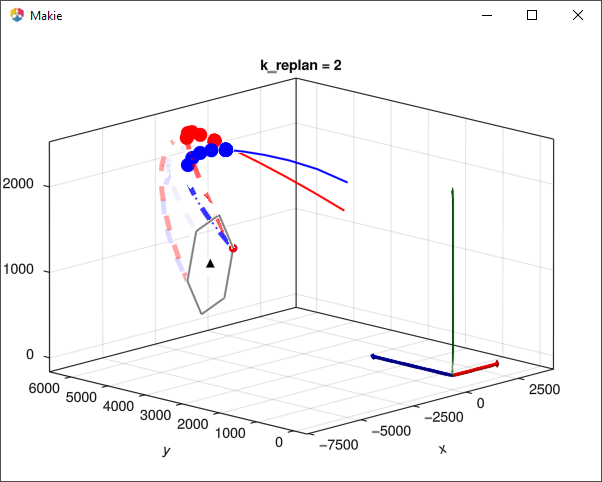
\includegraphics[width=\textwidth]{images/k_replan_1.png}
        \caption{Second replanning period.}
        \label{fig:first}
    \end{subfigure}
    % \hfill % Adds horizontal space between the two images
    \begin{subfigure}[b]{0.31\textwidth}
        \centering
        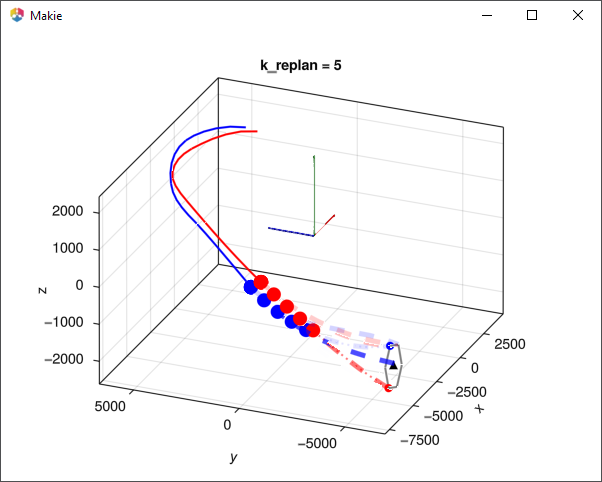
\includegraphics[width=\textwidth]{images/k_replan_5.png}
        \caption{Fifth replanning period.}
        \label{fig:second}
    \end{subfigure}
    \begin{subfigure}[b]{0.31\textwidth}
        \centering 
        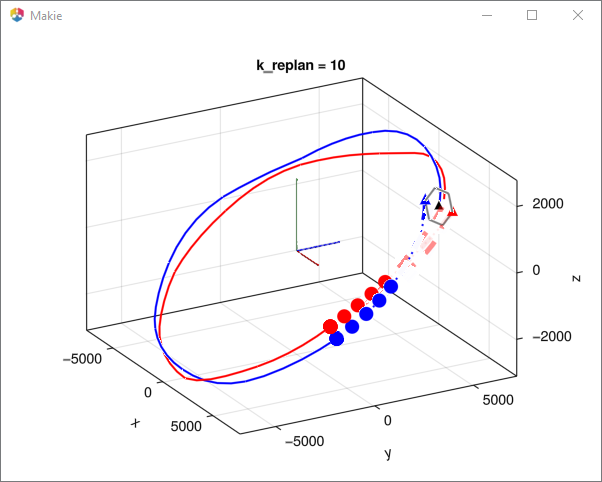
\includegraphics[width=\textwidth]{images/k_replan_10.png}
        \caption{Tenth (and final) replanning period.} 
    \end{subfigure}
    \caption{\textbf{Propagated and mixed trajectories at the the 2nd, 5th, and 10th replanning periods.} The solid lines represent the trajectories already traveled during past planning periods. For the current planning period, the dots represent the propagated (and chosen) trajectories, and the dashed lines represent the candidate trajectories. The darkness of the dashed lines represent the weights associated with each trajectory. }
    \label{fig:main_figure}
\end{figure*}

Then, we compute trajectories targeting the 6 vertices of the polygon for the pursuer and the evader. 
The stage cost at each time instant was computed and then averaged along the entire trajectory. 
\begin{equation}
    c(t) = \sqrt{ || \mathbf{r}_1(t) - \mathbf{r}_2(t) ||_2 + \lambda_1 } + \lambda_2 ( || \mathbf{u}_1(t) ||_2 - || \mathbf{u}_2(t) ||_2 )
\end{equation} 
The average stage cost was then saved in a cost matrix for each trajectory / vertex pairing. This results in a 6x6 cost matrix for each player. 

We are playing a zero sum game, so the cost matrix for one player is equivalent to the negative of the cost matrix for the other player. 

To solve the mixed strategy problem and find weights for each trajectory, we first transform the game to ensure that the cost matrix is entrywise positive. 

Then, we solve the simplex linear program associated with a zero sum game. 
% 
\begin{align}
    \max_{ \mathbf{z} \in \mathbb{R}^6 }    & \; \; \mathbf{1}^T \mathbf{z} \\ 
    \text{ subject to }                     & \; \; \mathbf{1} \geq A^T \mathbf{z}    
\end{align} 

Finally, we transform the solution into a probability simplex. This results in mixing weights $ x^* $ for each trajectory / vertex for each player. 

\begin{equation}
    x^* = \frac{\mathbf{z^*}}{ \mathbf{1}^T \mathbf{z^*} }  
\end{equation} 

To play the game, we sample from the mixing weights for each player. To construct the initial guess for the control input, we compute the initial velocity vector required for a Lambert transfer. We divide the velocity into 10 segments for each planning period of the trajectory to set as the initial guess vector. 

% \begin{figure*}[!t]
%     \centering
%     \begin{subfigure}{0.48\linewidth}
%         \centering
%         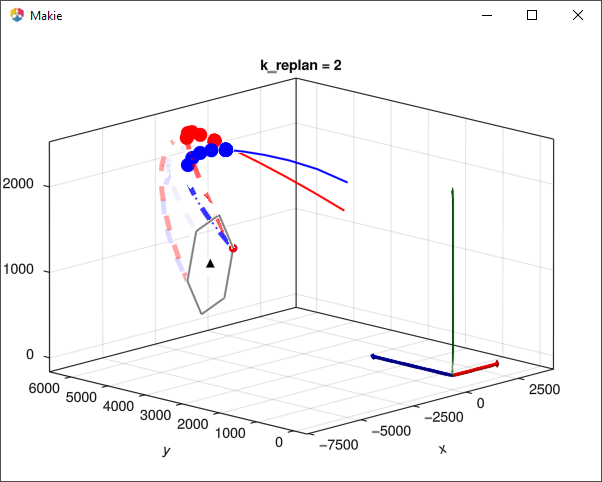
\includegraphics[width=\linewidth]{images/k_replan_1.png}
%         \caption{Body rates $\omega_{body}$ (rad/s) }
%         \label{fig:omega_bus} 
%     \end{subfigure}
%     \hfill
%     \begin{subfigure}{0.48\linewidth}
%         \centering
%         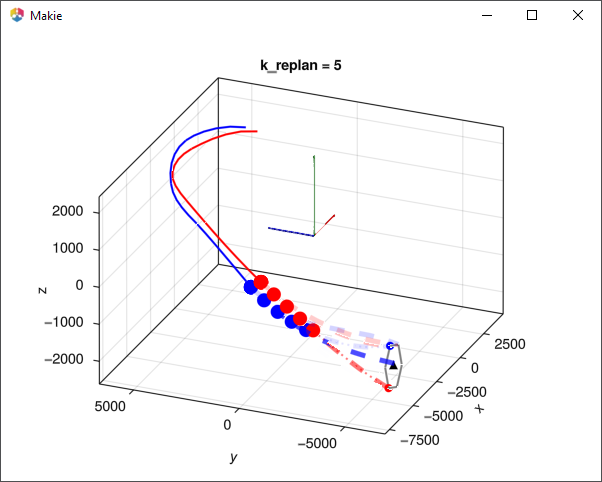
\includegraphics[width=\linewidth]{images/k_replan_5.png}
%         \caption{Body rates $\omega_{body}$ FFT }
%         \label{fig:omega_bus_fft} 
%     \end{subfigure}
%     \caption{asdf} 
%     \label{fig:cgs_rigid_body} 
%     \vspace{-1em}
% \end{figure*}

\begin{equation}
    \boldsymbol{v}_1, \boldsymbol{v}_2 = 
    % minLambert
    \operatorname{Lambert}
    (\boldsymbol{r}^P_0, \boldsymbol{r}^E_0, t_2, t_1, \mu). \label{eq:min_lambert}
\end{equation} 

\begin{figure}[ht!]
    \centering
    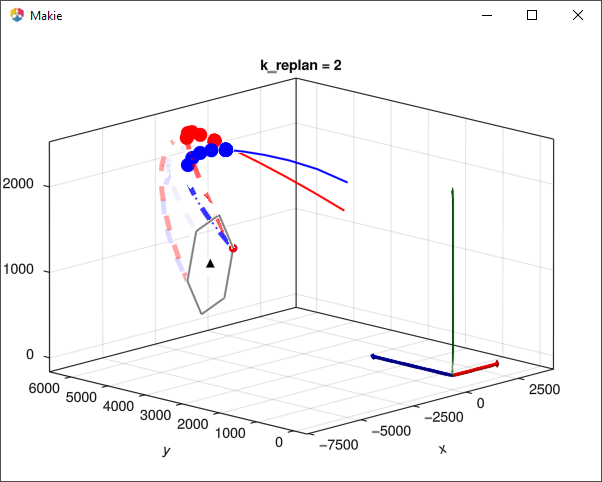
\includegraphics[width=0.9\linewidth]{images/k_replan_1.png}
    \caption{Caption}
    \label{fig:enter-label}
\end{figure}

% \begin{figure}[ht!]
%     \centering
%     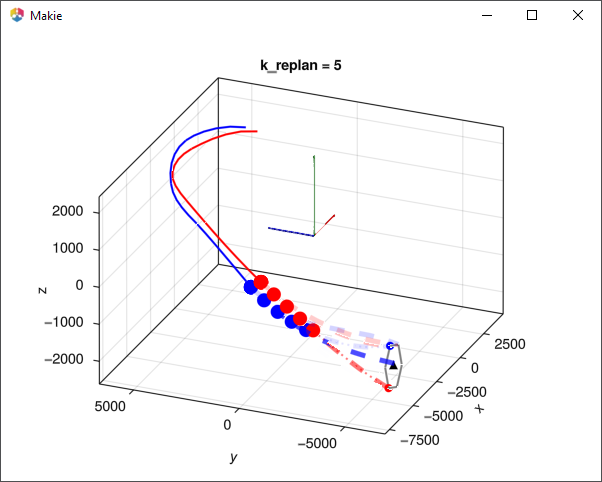
\includegraphics[width=0.9\linewidth]{images/k_replan_5.png}
%     \caption{Caption}
%     \label{fig:enter-label}
% \end{figure}

% \begin{figure}[ht!]
%     \centering
%     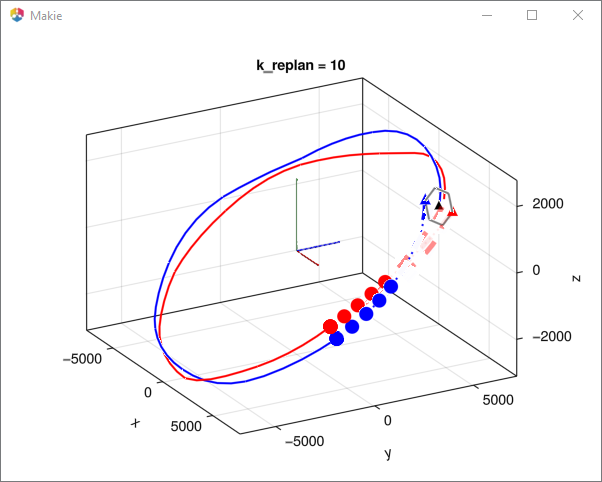
\includegraphics[width=0.9\linewidth]{images/k_replan_10.png}
%     \caption{Caption}
%     \label{fig:enter-label}
% \end{figure}








% % ================================================== % 

\section{Experiments \& Results}
\label{sec:results}


\begin{figure}
    \centering
    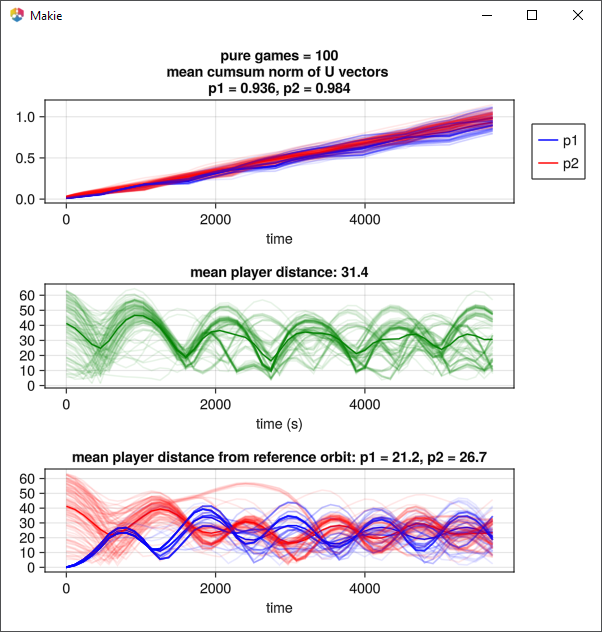
\includegraphics[width=0.9\linewidth]{images/pure.png}
    \caption{Pure Games}
    \label{fig:enter-label}
\end{figure}

\begin{figure}
    \centering
    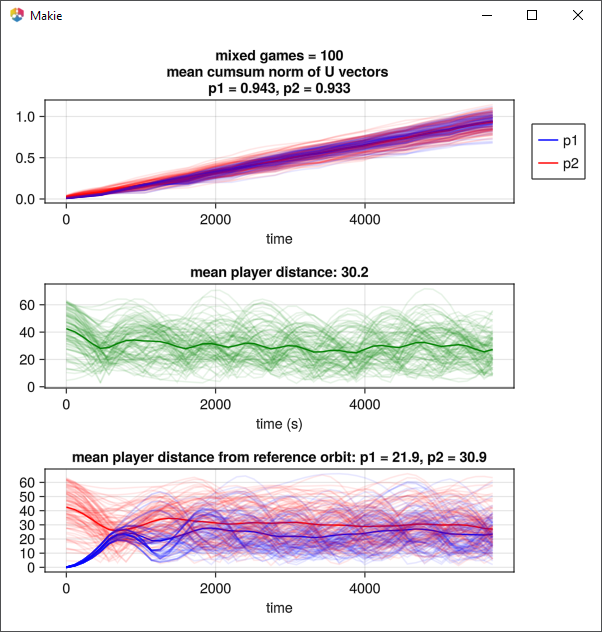
\includegraphics[width=0.9\linewidth]{images/mixed.png}
    \caption{Mixed Games}
    \label{fig:enter-label}
\end{figure}

\begin{figure}
    \centering
    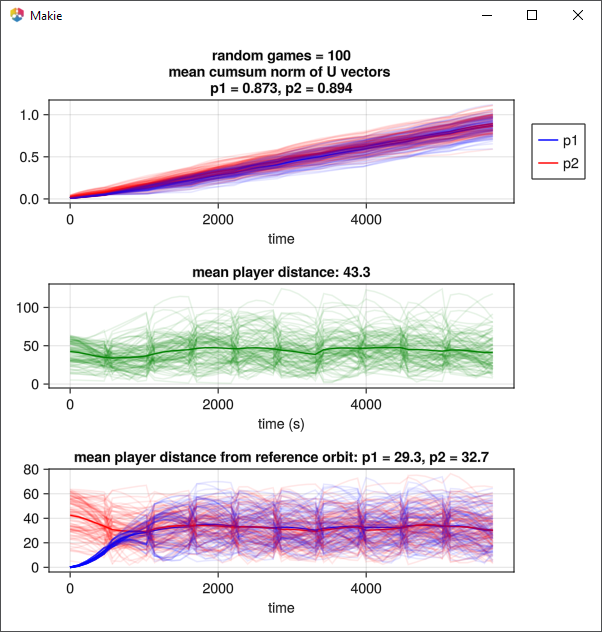
\includegraphics[width=0.9\linewidth]{images/random.png}
    \caption{Random Games}
    \label{fig:enter-label}
\end{figure}




% % ================================================== % 

% \section{Conclusions \& Future Work}
\section{Discussion}
\label{sec:conclusions}
\input{sections/conclusions}



% ================================================== % 
\addtolength{\textheight}{-12cm}   % This command serves to balance the column lengths
                                  % on the last page of the document manually. It shortens
                                  % the textheight of the last page by a suitable amount.
                                  % This command does not take effect until the next page
                                  % so it should come on the page before the last. Make
                                  % sure that you do not shorten the textheight too much.

% ================================================== % 


% \balance
% \printbibliography
\bibliographystyle{ieeetr}
\bibliography{refs}


% ================================================== % 
\end{document}
